\chapter{Wstęp}
\label{cha:wstęp}
Morfologia krwi (ang. \textit{complete blood count}) jest jednym z najczęściej przeprowadzanych badań. Dostarcza ona informację o komórkach krwi pacjenta, w tym liczbę komórek każdego typu krwinek i wartość stężenia hemoglobiny. Zgodnie z zaleceniami powinno się wykonywać je przynajmniej raz do roku w celach profilaktycznych. Jest to też jedno z pierwszych badań stosowanych w diagnostyce schorzeń. Według reportu GUS 42\% osób decydujących się na badanie labolatoryjne wybiera właśnie badanie krwi (\ref{GUS_Zdrowie2016}), \cite{GUS_Zdrowie2016}.

\begin{figure}[h]
\begin{center}
	\begin{tikzpicture}[scale = 0.8]
		\pie [polar, explode=0.1, text=legend] 
    		{42/badania krwi,
     	36/badania moczu,
     	9/cytologia, 
     	2/PSA, 
     	11/inne}
	\end{tikzpicture}
\end{center}
\caption{Typy wykonanych badań labolatoryjnych według GUS.}
\label{GUS_Zdrowie2016}
\end{figure}

{\parindent0pt % disables indentation for all the text between { and }
Biorąc pod uwagę stan ludności i ograniczoną liczbę personelu medycznego w szpitalach maualne wykonywanie tego typu badań jest problematyczne i zajmuje dużo czasu. Poprzez usunięcie czynnika ludzkiego można uzyskać większą poprawność i zwiększyć poduktywność personelu medycznego. Celem pracy jest zbudowanie narzędzia do automatycznej klasyfikacji białych krwinek opartego na głęboko uczonych konwolucyjnych sieciach neuronowych. Na wejściu do sieci wprowadzane są zdjęcia pojedynczych krwinek, wykonane pod mikroskopem. W tym celu została wykorzystana baza danych na licencji MIT, zawierająca cztery klasy krwinek najliczniej występujące w składzie krwi. Każde zdjęcie jest oryginalnie przyporządkowane do odpowiedniej klasy, zgodnie z widniejącym na nim elementem morfologicznym. 

Przed użyciem bazę podzielono na rozłączne zbiory: uczący, walidacyjny i testowy. Za pomocą zbiorów uczącego i walidacyjnego przetrenowano i nastrojono klasyfikator. Dzięki danym ze zbioru testowego, zawierającego zdjęcia nigdy nie wprowadzane na wejście sieci, sprawdzono skuteczność zastosowanej metody.

Oczekiwanym wynikiem pracy jest zbudowanie sieci neuronowej określającej z jak najlepszą doładnośćią jaki typ krwinki znajduje się na zdjęciu, a następnie modyfikacja zarówno parametrów sieci jak i danych wejściowych w celu zbadania wpływu zmian na działanie modelu.

Program został napisany w języku Python, który jest dobrze przystosowany do przetwarzania, analizy i modelowania danych. Do implementacji sieci użyta została biblioteka Keras, która jest wysokopoziomowym API biblioteki TensorFlow.
}
%---------------------------------------------------------------------------
\section{Motywacja pracy}
\label{sec:motywacja_pracy}

W celu prawidłowego zdiagnozowania chorób często konieczne jest zbadanie liczby krwinek białych danego typu. Obecnie proces ten jest wykonywany manualnie za pomocą hemocymetru (\ref{blood_cells_microscope}) lub automatycznie z użyciem np. technologii VCS, pomiarem impedancji czy pomiarami z użyciem laseru. 

\begin{figure}[h]
	\centering
		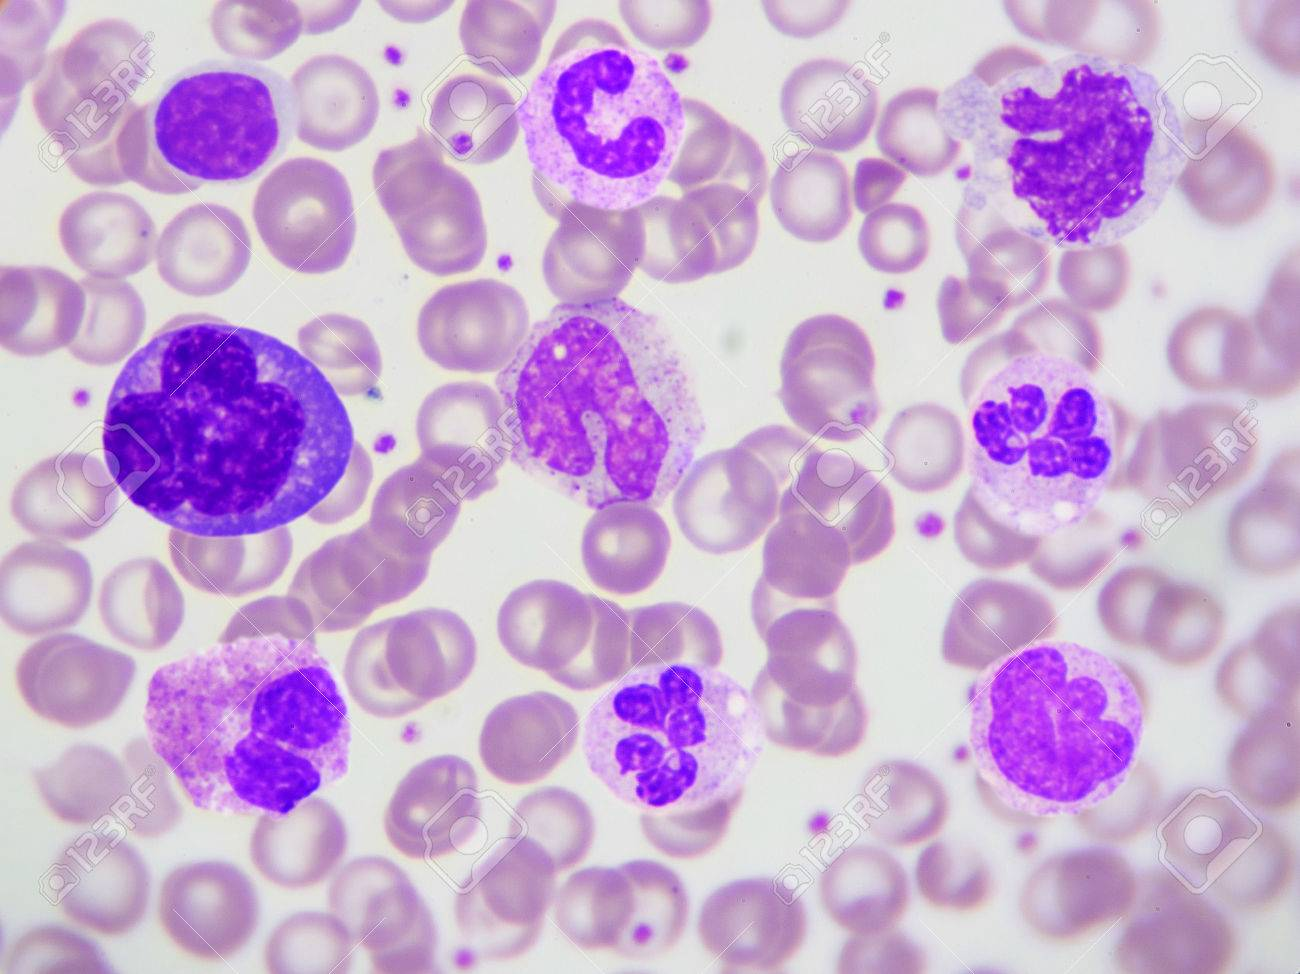
\includegraphics[scale=0.6]{blood_cells_microscope}
	\caption{Widok krwinek badanych pod mikroskopem \cite{cells_microscope}.}
	\label{blood_cells_microscope}
\end{figure}

{\parindent0pt % disables indentation for all the text between { and }
Ciekawą alternatywą dla tych metod byłoby zastosowanie automatycznego zliczania komórek opartego na klasyfikacji przynależności do danego typu na podstawie analizy obrazów przez sieć neuronową. Byłaby to metoda nie wymagająca ingerencji czynnika ludzkiego, jak to ma miejsce w przypadku badania manualnego, a jednocześnie tańsza niż stosowane pomiary automatyczne. Zmniejszenie liczby ręcznych procesów i nadmiaru próbek podczas rutynowych badań zwolniłoby miejsce dla innych ważnych zadań, zwiększyło wydajność i poprawiło jakość analiz. W pełni zautomatyzowany proces zmniejszyłby indywidualne ryzyko błędów.

Bazą do zbudowania takiego narzędzia byłaby sieć rozpoznająca typ krwinki na zdjęciu i właśnie tą częścią zajmuje się niniejszy projekt. W pracy zdecydowano się na sieć konwolucyjną głęboko uczoną i w zależności od parametrów zbadano precyzyjność jej działania. W tym celu przetestowano wiele kombinacji doboru składowych modelu, a poniżej opisano kilka najciekawszych przypadków.
}
%---------------------------------------------------------------------------
\section{Cel i zrealizowane zadania}
\label{sec:cel_i_zrealizowane_zadania}

Aby zbudować narzędzie do klasyfikacji krwinek białych najpierw przeprowadzono analizę przydatności takiego rozwiązania na rynku oraz sprawdzono jakie metody są obecnie wykorzystywane w badaniach krwi. Analiza wykazała zasadność stworzenia tego typu automatyzacji.

{\parindent0pt % disables indentation for all the text between { and }
Następnym krokiem było zapoznanie się ze stanem obecnej wiedzy na temat sieci neuronowych głęboko uczonych oraz sieci konwolucyjnych i przegląd dostępnych rozwiązań podobnych problemów. Po wyciągnięciu wniosków z zebranych informacji przystąpiono do planowania i implementacji modelu sieci. Wybrano model osiągający najlepsze wyniki i przystąpiono do badania wpływu doboru jego parametrów na dokładność klasyfikacji.

Wynikiem końcowym pracy jest klasyfikator osiągający X\% skuteczność na zbiorze testowym oraz wnioski wyciągnięte z badań nad zależnością skuteczności od doboru hiperparametrów.
}
%---------------------------------------------------------------------------
\section{Zawartość pracy}
\label{sec:zawartosc_pracy}

W rodziale~\ref{cha:analiza_problemu_badawczego} przedstawiono teoretyczną analizę problemu badawczego wraz z kilkoma przykładowymi rozwiązaniami zadania klasyfikacji wizyjnej na podstawie najnowszych publikacji. 

{\parindent0pt % disables indentation for all the text between { and }
Rozdział~\ref{cha:system_do_klasyfikacji_elementow_morfologicznych} zawiera opis implementacji programu i zastosowanych metod, zaś rozdział~\ref{cha:analiza_wynikow} zestawienie i analizę uzyskanych wyników, po którym następuje podsumowanie przeprowadzonego badania.
}